\subsection{Architecture}

Our product it made up of two parts: the control server, and the door nodes.
Our product interacts with two types of actors: Operators and Users.

The control server maintains a database of operator profiles, operator logs,
user profiles, and interaction logs.  The control server will use the operator
profiles to validate users using the operator GUI.  Every action performed in
the operator GUI will be logged in the operator logs.  Operators can create and
modify user profiles.  When a user attempts to use a door node, their identity
is checked against their user profile.  Each interaction with a door node is
recorded in a user log.

\begin{figure}[!htb]
\centering
\includegraphics[width=\textwidth]{figures/architecture.png}
\caption{UML Architecture Diagram}
\label{fig:architecture-diagram}
\end{figure}

\subsection{Communication Protocol}

\begin{itemize}
\item Account ID: (number) uniquely identifies an account
\item Node ID: (number) uniquely identifies a door node
\item Transaction ID: (number) uniquely identifies a transaction
\item Current time: (number) Time message was sent
\item Information Request: (list of keys) A list of information required to further the
transaction
\item Information Response: (list of key value pairs) Contains obtained information
\item Access Request Response: (boolean)
\end{itemize}

\begin{table*}[htb]
\begin{tabular}{ l | l | l | p{4.5cm} }
\toprule
Sender & Receiver & Message & Data Format\\
\midrule
Door Node & Control Server & ACCESS\_REQUEST &
Node ID \newline Transaction ID \newline Current time \newline Account ID\\
\hline
Door Node & Control Server & INFORMATION\_RESPONSE &
Node ID \newline Transaction ID \newline Current time \newline Information Response\\
\hline
Control Server & Door Node & INFORMATION\_REQUEST &
Node ID \newline Transaction ID \newline Current time \newline Information Request\\
\hline
Control Server & Door Node & ACCESS\_RESPONSE &
Node ID \newline Transaction ID \newline Current time \newline Account ID \newline Access Request Response\\
\bottomrule
\end{tabular}
\caption{Messages}
\end{table*}

\subsection{Message Sequence Diagrams}

\begin{figure}[!htb]
\centering
\includegraphics[width=\textwidth]{figures/message-sequence-diagram.png}
\caption{Message Sequence Diagram}
\label{fig:message-sequence-diagram}
\end{figure}

\subsection{Database Schema}

\begin{figure}[!htb]
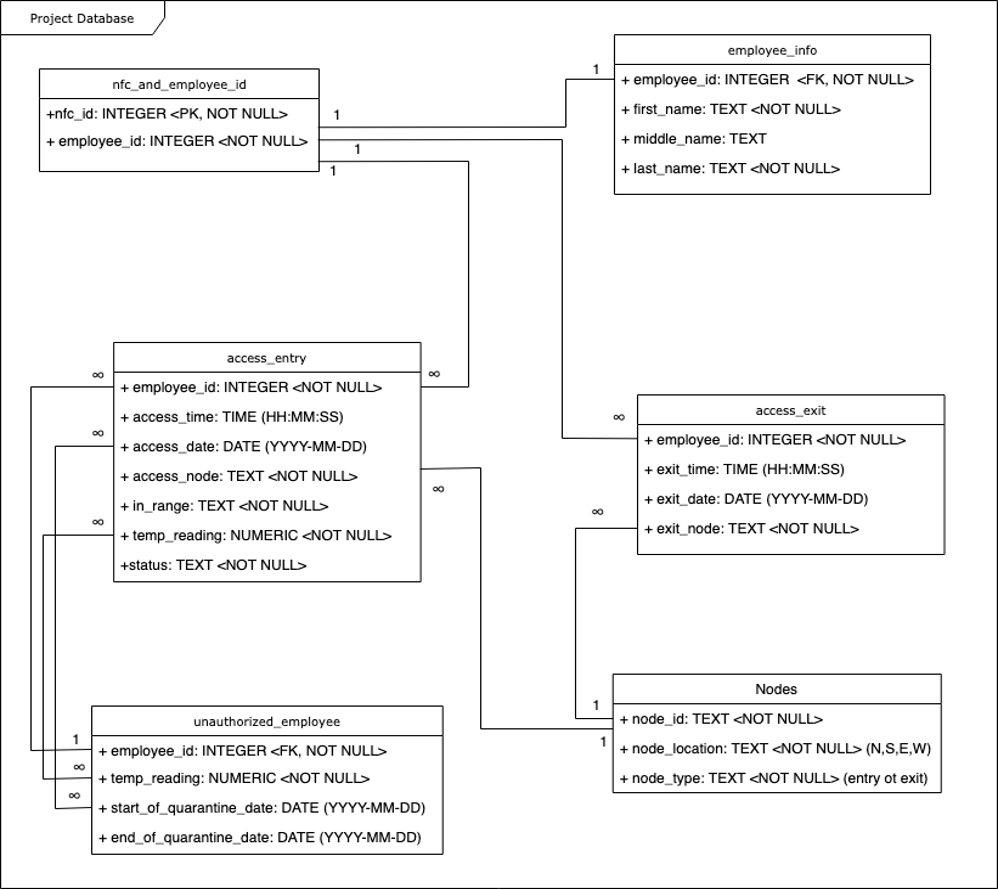
\includegraphics[width=\textwidth]{figures/db-schema.png}
\caption{Database Schema}
\end{figure}

